\subsection{\texorpdfstring{Channel \& Graph}{Channel and Graph}}

\subsubsection*{Channel}

      \begin{frame}
            \frametitle{Channel}
            \begin{definition}[channel]
                  A channel has a sender and a receiver.
                  \pause


                  A message is a finite sequence of characters.
                  The sender sends a message to the receiver.
                  \begin{figure}[h!]
                        \tikzstyle{vertex}=[fill=black!25,minimum size=20pt,inner sep=0pt]
                        \tikzstyle{message}=[inner sep=0pt]
                        \tikzstyle{edge} = [draw,thick,-]
                        \tikzstyle{weight} = [font=\small]
                        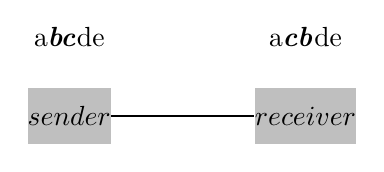
\begin{tikzpicture}[scale=1, auto,swap]
                              % Draw a 7,11 network
                              % First we draw the vertices
                              \foreach \pos/\name in {{(0,0)/sender}, {(3,0)/receiver}}
                                    \node[vertex] (\name) at \pos {$\name$};
                              \foreach \pos/\name/\la in {{(0,1)/abcde/a\textbf{\textit{bc}}de}, {(3,1)/acbde/a\textbf{\textit{cb}}de}}
                                    \node[message] (\name) at \pos {\la};
                              % Connect vertices with edges and draw weights
                              \foreach \source/ \dest in {sender/receiver}
                              \path[edge] (\source) -- node[weight]{} (\dest);
                        \end{tikzpicture}
                  \end{figure}
                  \pause
                  
                  The receiver receives message and decode it.
                  \pause

                  However, in the procedure of send and receive, the channel may introduce some errors. For instance, here, character $b$ is decoded into $c$. 
            \end{definition}
      \end{frame}

\subsubsection*{Confusable}

      \begin{frame}
            \frametitle{Confusable}
            \begin{definition}[confusable]
                  Given two distinct characters $a$, $b$. If $a$ and $b$ have chance to be decoded into a same character say $c$, we say $a$ and $b$ are confusable.

                  For a two distinct messages of length $n$, say $a_{1}a_{2}\dots a_{n}$, $b_{1}b_{2}\dots b_{n}$ is confusable if and only if $a_{i}$ and $b_{i}$ are \textbf{confusable} or \textbf{same} for every $i$.
            \end{definition}
      \end{frame}

\subsubsection*{Rate of Channel}

      \begin{frame}
            \frametitle{Rate of Channel}

            \begin{definition}[rate of channel]
                  The rate of channel actually represent how many distinct character can be send per unit time.

                  Given a channel that could send $r$ distinct characters per unit time. And send message for $n$ unit time, so the number of distinct messages the channel can send is $r^{n}$.

                  \pause

                  Conversely, given a channel that could send $m$ distinct messages in $n$ unit time.
                  The rate of channel is $\sqrt[n]{m}$.
                  
            \end{definition}
      \end{frame}

\subsubsection*{Zero Error Rate of Channel}

      \begin{frame}
            \frametitle{Zero Error Rate of Channel}
            \begin{definition}[zero error rate]
                  Given a channel that could send messages in $n$ unit time.

                  We want to find the maximum set of messages $M$ that no two of them is confusable.

                  \begin{equation}
                        \text{zero error rate} = \max_{M} \sqrt[n]{|M|}
                  \end{equation}
            \end{definition}
      \end{frame}

      \begin{frame}
            \frametitle{Zero Error Rate of Channel}
            If given a set of characters $S$, and some of the characters could be confusable.

            We want to find
            \begin{equation}
                  \sup_{n} \left\{
                        \text{zero error rate of channel send messages for $n$ unit time}
                  \right\}
            \end{equation}

            And we call this the shannon Capacity and denoted by $\Theta(S)$.

            Clearly, shannon Capacity is actually a function of the set of characters. So, we want a more abstract way to represent the characters.
      \end{frame}

\subsubsection*{Graph}

\begin{frame}
      \frametitle{Graph Representation Of Characters}
      \begin{definition}[graph] \label{def:graph}
            A graph $ G $ is a set of vertices with a set of edges connecting pairs of vertices.

            \begin{figure}[h!]
                  \tikzstyle{vertex}=[circle,fill=black!25,minimum size=20pt,inner sep=0pt]
                  \tikzstyle{edge} = [draw,thick,-]
                  \tikzstyle{weight} = [font=\small]
                  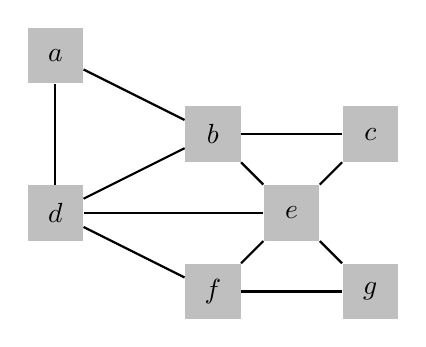
\begin{tikzpicture}[scale=1, auto,swap]
                        % Draw a 7,11 network
                        % First we draw the vertices
                        \foreach \pos/\name in {{(0,2)/a}, {(2,1)/b}, {(4,1)/c},
                              {(0,0)/d}, {(3,0)/e}, {(2,-1)/f}, {(4,-1)/g}}
                              \node[vertex] (\name) at \pos {$\name$};
                        % Connect vertices with edges and draw weights
                        \foreach \source/ \dest in {b/a, c/b,d/a,d/b,
                              e/b, e/c,e/d,
                              f/d,f/e,
                              g/e,g/f}
                        \path[edge] (\source) -- node[weight]{} (\dest);
                  \end{tikzpicture}
                  \label{fig:graphDefinitionExample}
                  \caption{An example of a graph.}
            \end{figure}
      \end{definition}
\end{frame}

\begin{frame}
      \frametitle{Graph Representation Of Characters}
      \begin{definition}\label{def:graphRepresetationOfChannel}
            Given a channel that sending $\{1,2,\dots,n\}$ as characters. And some characters $i$ and $j$ could be confused with each other.

            \smallskip

            Then the graph representation of the characters is the graph with vertices $\{1,2,\dots,n\}$ and edges $(i,j)$ if and only if $i$ and $j$ is distinct and could be confused with each other.
      \end{definition}

      Accordingly, there is the corresponding way that using graphs to represent a message and Shannon Capacity.
\end{frame}

\begin{frame}
      \frametitle{Product Graph}
      \begin{definition}[graph product]\label{def:graphProduct}
            The product of two graphs can be considered as send a pair of characters $(x,y)$ as one message. So, we have a channel that send messages of for $2$ unit time.

            \pause
            \smallskip

            Recall that before, $2$ distinct messages is confusable means that they can be decoded into the same message, which means every characters the two channel use need to be confusable or the same.

            \smallskip

            Given two graph $ G $ and $ H $. The graph product $ G \times H $ is the graph with vertices $ V(G \times H) = V(G) \times V(H) $ in which $ (x,y) $ is adjacent to $ (x',y') $ in $ G \times H $ if and only if $ x $ is \textbf{adjacent} to $ x' $ or the \textbf{same} in $ G $ and $ y $ is \textbf{adjacent} to $ y' $ or the \textbf{same} in $ H $.

            \pause

            A graph $ G $ product itself for $ n $ times will always be denoted by $ G^n $.

            Which means we could use $ G^n $ to represent messages of a channel that send messages for $n$ unit time.
      \end{definition}
\end{frame}

\begin{frame}
      \frametitle{$\alpha(G)$}
      \begin{definition}[$\alpha(G)$]\label{def:alpha}
            Given a finite graph $G$. $\alpha(G)$ is the \textbf{maximum} number of vertices of the subgraph of $G$ such that every vertex of the subgraph is not adjacent in $G$.

            If $G$ represent a set of characters, $\alpha(G^{n})$ is just the zero error rate we have defined before.

            \pause

            \tikzstyle{vertex}=[circle,fill=black!25,minimum size=20pt,inner sep=0pt]
            \tikzstyle{selected vertex}=[circle,fill=red!25,minimum size=20pt,inner sep=0pt]
            \tikzstyle{edge} = [draw,thick,-]
            \tikzstyle{weight} = [font=\small]
            \begin{figure}[h!]
                  \begin{tikzpicture}[scale=1, auto,swap]
                        % Draw a 7,11 network
                        % First we draw the vertices
                        \foreach \pos/\name in {{(0,1)/a}, {(2,1)/b}, {(4,1)/c},
                              {(0,0)/d}, {(3,0)/e}, {(2,-1)/f}, {(4,-1)/g}}
                              \node[vertex] (\name) at \pos {$\name$};
                        \foreach \pos/\name in {{(0,1)/a}, {(4,1)/c},
                              {(2,-1)/f}}
                              \node[selected vertex] (\name) at \pos {$\name$};
                        % Connect vertices with edges and draw weights
                        \foreach \source/ \dest in {b/a, c/b,d/a,d/b,
                              e/b, e/c,e/d,
                              f/d,f/e,
                              g/e,g/f}
                        \path[edge] (\source) -- node[weight]{} (\dest);
                  \end{tikzpicture}
                  \label{fig:alphaGExample}
                  \caption{Example of $ \alpha(G) $. Here $ \alpha(G) = 3 $.}
            \end{figure}
      \end{definition}
\end{frame}
